% !TEX root= ...main.tex

\section{Функциональное назначение программы}

\subsection{Назначение программы}

%
\textbf{GIS Excelsior} предназначена для планирования колонизации планеты Марс. Под планированием подразумевается:

\begin{itemize}
	\item Выбор участка поверхности Марса для размещения колонии;
	\item Размещение зданий и модулей различного назначения на выбранном участке поверхности планеты с учетом соответствующих критериев размещения перечисленных в Таблице~\ref{tab:criterions}.
	\item Ознакомление с перечнем доступных для размещения объектов, их описанием и уровнями из таблицы критериев.
\end{itemize}
%



\subsection{Работа с интерфейсом}

%
При запуске сайта перед вами должен появиться следующий интерфейс:

\begin{figure}[h!]
	\centering
	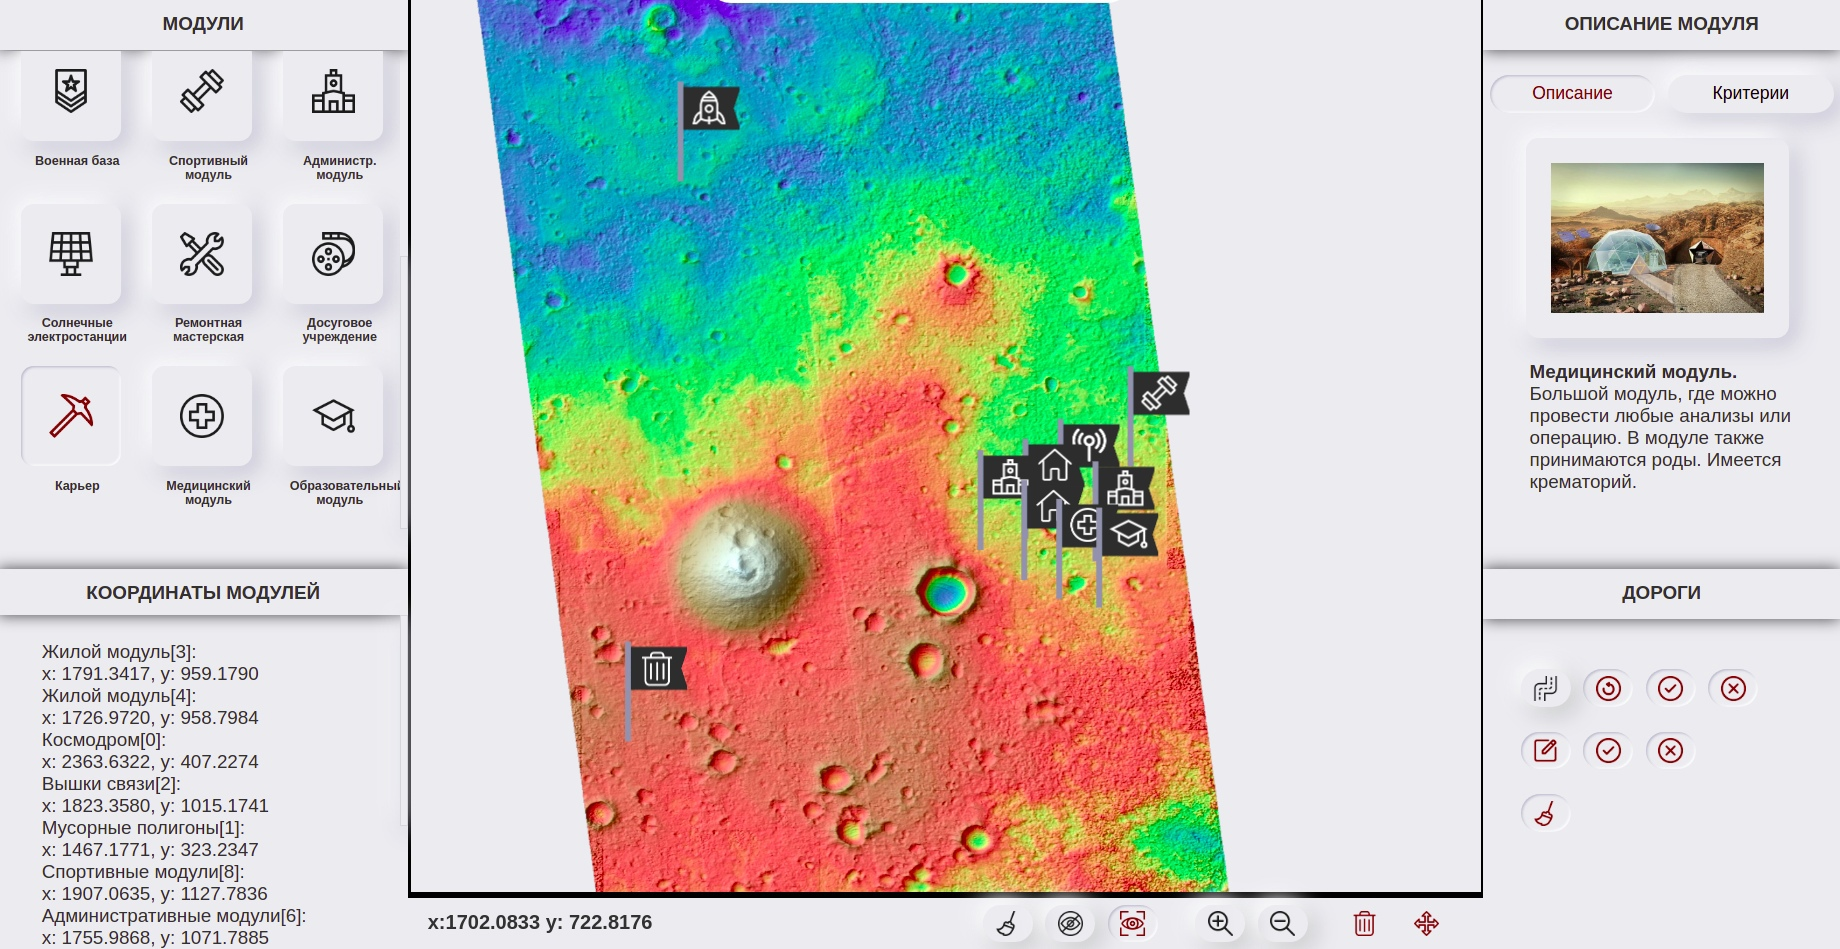
\includegraphics[width=.9\linewidth]{./img/interface}
	\caption{Общий вид интерфейса программы}\label{fig:interface}
\end{figure}

Самая главное, что вы должны видеть -- это участок поверхности Марса в \textbf{RGB} расцветке. Весь интерфейс можно разделить на 5 частей:

\begin{enumerate}
	\item \textbf{Центральная часть.} Здесь расположена карта,  инструменты для работы с размещенными на ней объектами, а также отображаются координаты точки под курсором.
	\item \textbf{Левый верхний угол.} Этот блок позволяет вам выбирать объект, который вы хотите разместить на карте.
	\item \textbf{Левый нижний угол.} Здесь будет появляться информация о размещенных объектах, их наименованиях и координаты.
	\item \textbf{Правый верхний угол.} В этом блоке вы можете заметить две вкладки: \textbf{<<Описание>>} и \textbf{<<Критерии>>}. Во вкладке <<Описание>> отображается фото с внешним видом выбранного объекта. Во вкладке <<Критерии>> написаны уровни критериев, которым соответствует выбранный объект.
	\item \textbf{Правый нижний угол.} В последнем блоке можно найти инструменты для размещения и редактирования дорог.
\end{enumerate}

Поговорим про каждый блок подробнее. В следующих параграфах.

\subsubsection*{Карта}

На карте вы можете разместить объекты из левого верхнего блока, а также ,,построить`` дороги используя возможности правой нижней части интерфейса. Карта раскрашена в \textbf{RGB} расцветке по высотам. Высоты растут от синего цвета к красному и белому.

\begin{wrapfigure}{r}{.4\linewidth}
	\centering
	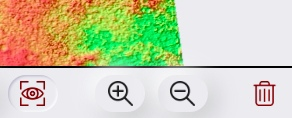
\includegraphics[width=.9\linewidth]{./img/zoom}
	\caption{Инструменты для изменения масштаба карты}\label{fig:zoom}
\end{wrapfigure}

Карту можно перемещать как вам удобно используя левую кнопку мыши (ЛКМ): наведите на карту, зажмите ЛКМ и перемещайте курсор не отпуская кнопку. Таким образом вы можете разместить нужный участок карты, например в центр.

Также можно использовать колесо мыши для приближения и отдаления (zoom) карты. Помимо этого вы можете кликать ЛКМ на соответствующие инструменты под картой, которые обозначены как две лупы (см.~рис.~\ref{fig:zoom}).

\begin{figure}[h!]
	\centering
	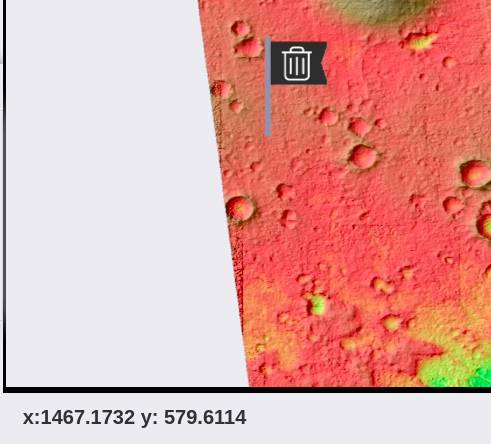
\includegraphics[width=.45\linewidth]{./img/coordinates}
	\caption{Отображение координат точки под курсором}\label{fig:coordinates}
\end{figure}

Можно заметить, что при наведении курсора на карту, в левом нижнем углу центрального окна видны координаты позиции (см.~рис.~\ref{fig:coordinates}). При перемещении курсора их можно отслеживать в реальном времени.

На панели инструментов под картой можно найти следующие инструменты: 

\begin{enumerate}
	\item \textbf{Очистить.} Очищает всю карту от любых объектов. \underline{Необратимое} действие.
	\item \textbf{Скрыть.} Скрывает все объекты карты, кроме дорог.
	\item \textbf{Показать.} Если какие-то объекты были скрыты, после нажатия этой кнопки они вернутся на карту.
	\item \textbf{Приблизить.} Уменьшает масштаб карты: все объекты становятся крупнее, а площадь обозреваемой поверхности уменьшается.
	\item \textbf{Отдалить.} Увеличивает масштаб карты: все объекты становятся меньше, а площадь обозреваемой поверхности увеличивается.
	\item \textbf{Удалить.} Удалить выбранный объект на карте. \underline{Необратимое} действие.
	\item \textbf{Переместить.} Переместить выбранный объект в другое место.
\end{enumerate}



\subsubsection{Блок <<Модули>>}

Блок <<Модули>> -- это панель, где есть только предлагаемые программой модули, которые вы можете разместить на карте. Здесь вы можете найти следующие объекты:

\begin{enumerate}
	\item \textbf{Жилой модуль.} Небольшой модуль, может полноценно обеспечивать жилье для 6-10 колонистов, включает в себя кровати, ящики для хранения вещей, комнату для поддержания гигиены и т.д.
	
	\item \textbf{Космодром.} Достаточно обширная территория, где расположен ЦУП, взлетно-посадочные площадки, здания для обслуживания космодрома и проживания персонала, хранилища и центр сборки и ремонта ракет.
	
	\item \textbf{Центр связи.} Центр связи со спутниками, также позволяет связаться с удаленными объектами колонии.
	
	\item \textbf{Растительный модуль.} Модуль, где выращиваются и исследуются растения. В большинстве модулей выращивается пища для колонистов.
	
	\item \textbf{Мусорный полигон.} Открытое пространство, где выгружают мусорные отходы в виде контейнеров. На территории также расположен мусороперерабатывающий завод.
	
	\item \textbf{Производственное предприятие.} Перерабатывает сырье из карьеров, плантаций и др. в продукт (еду, материалы и изделия).
	
	\item \textbf{Военная база.} Служат для обеспечения безопасности колонии и сохраняют порядок в ней, то есть выполняют роль полиции в том числе.
	
	\item \textbf{Спортивный модуль.} Модуль который выполняет все функции небольшого спортзала, где колонисты могут поддерживать спортивную форму и не допускать атрофию мышц. 
	
	\item \textbf{Административный модуль.} Здесь работает управление колонией. Они планируют ее развитие, а также решают проблемы населения. В распоряжении модуля имеются все необходимые помещения, как совещательные комнаты, так и управляющие колонией специализированные помещения.
	
	\item \textbf{Солнечная электростанция.} Солнечные панели размещенные достаточно плотно. Вырабатывают электроэнергию и сохраняют ее в аккумуляторах. Полностью автоматическая система.
	
	\item \textbf{Ремонтная мастерская.} Ангар, где есть необходимое оборудование для починки любой вещи: от часов до марсоходов.
	
	\item \textbf{Досуговое учреждение.} Это могут быть кинокомнаты, теннисные корты, игровые и т.п. Здесь колонисты могут отвлечься от работы и отдохнуть. Найти себе хобби.
	
	\item \textbf{Карьер.} Удаленная от колонии территория, где добываются полезные ископаемые и грунт. Добытое сырье отправляется на перерабатывающие заводы.
	
	\item \textbf{Медицинский модуль.} Большой модуль, где можно провести любые анализы или операцию. В модуле также принимаются роды. Имеется крематорий.
	
	\item \textbf{Образовательный модуль.} Модуль, где помещается несколько классов. Имеются комнаты для занятий группами в любых сферах: от математики до астрономии.
\end{enumerate}

Наведя курсор на интересующий вас модуль и нажав ЛКМ, вы сможете выбрать его для размещения на карте, о чем вам подскажет соответствующая подсказка (см.~рис.~\ref{fig:choose_module}).

\begin{figure}[h!]
	\centering
	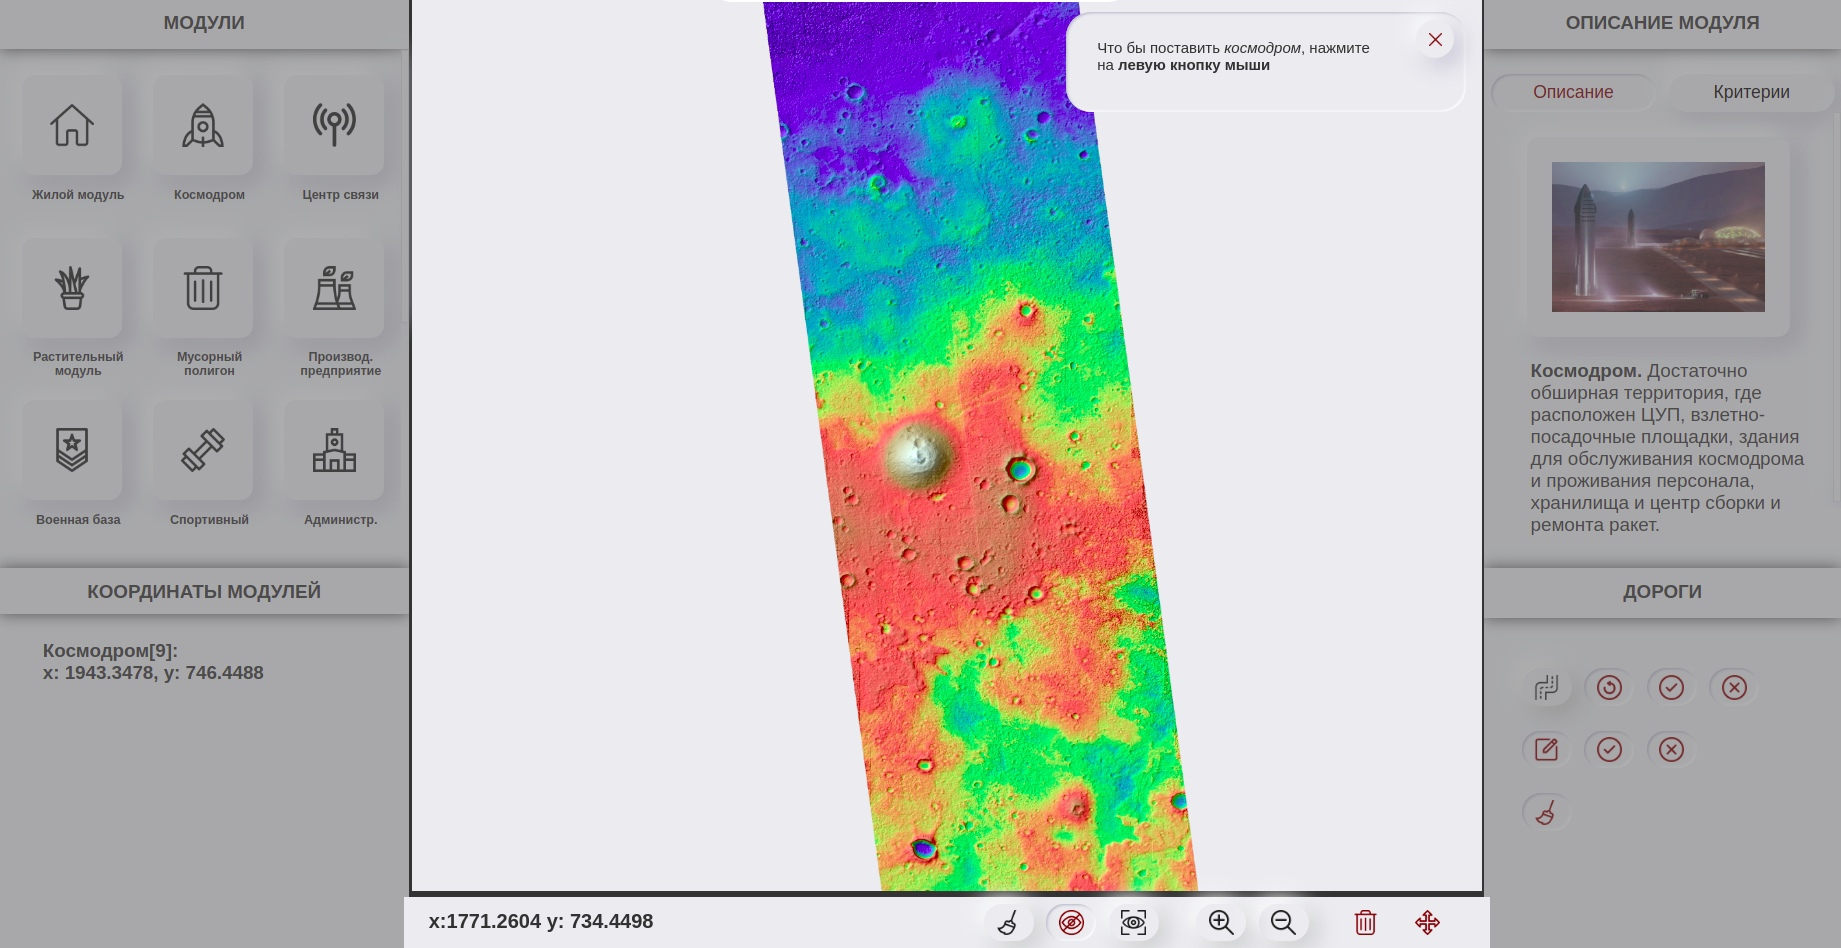
\includegraphics[width=\linewidth]{./img/choose_module}
	\caption{Размещение выбранного модуля на карте}\label{fig:choose_module}
\end{figure}

При размещении учитывается критерий \textit{опасность}, в виде красных окружностей, которые сигнализируют о зонах, в которых нельзя размещать ваш модуль. \textit{Примечание: красные зоны могут пересекаться.}

\begin{figure}[h!]
	\centering
	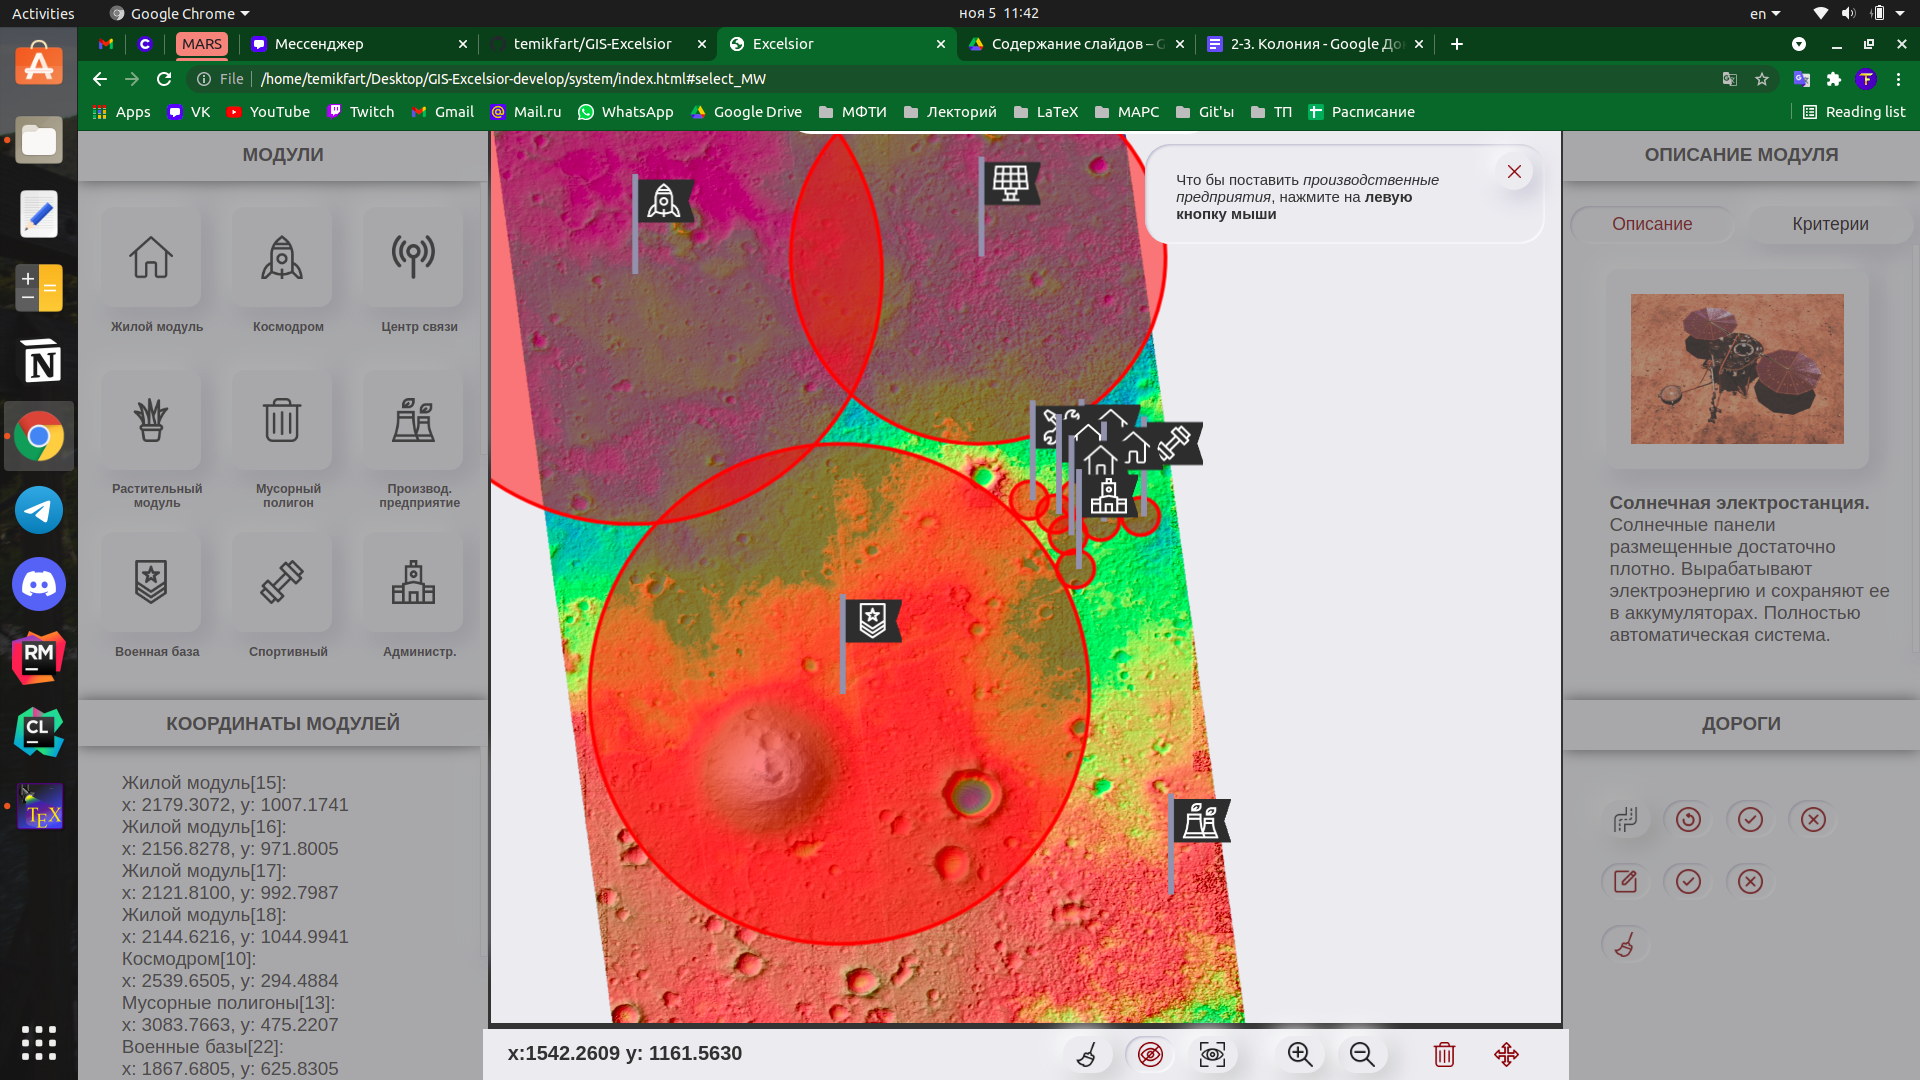
\includegraphics[width=.7\linewidth]{./img/red_zones}
	\caption{Демонстрация красных зон при размещении объектов}\label{fig:red_zones}
\end{figure}

Как видно из рис.~\ref{fig:red_zones}, красные зоны отлично помогают пользователю нашей программы знать, в какие места, точно нельзя располагать модуль.



\subsubsection{Блок <<Координаты модулей>>}

Здесь все предельно просто: при размещении очередного модуля на карту здесь появляется название модуля и его координаты. Такие отметки появляются последовательно. Если вы разместили модули в одной последовательности, в такой же вы увидите их и здесь. Это можно использовать для планирования, если для вас необходим сначала космодром, тогда разместите его первым, а после размещения других объектов скопируйте содержимое этого блока, чтобы знать что за чем следует.

\begin{figure}[h!]
	\centering
	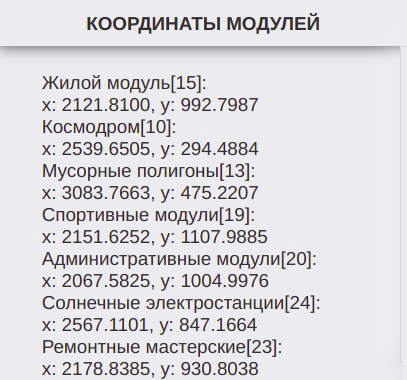
\includegraphics[width=.5\linewidth]{./img/module_coordinates}
	\caption{Демонстрация красных зон при размещении объектов}\label{fig:module_coordinates}
\end{figure}

Если же вы решите удалить какой-то объект с карты, тогда он пропадет из этого списка. Таким образом, вы можете быть уверены, что здесь записывается не история изменений.



\subsubsection{Блок <<Описание модулей>>}

Хоть этот блок и называется <<Описание модулей>>, но тут также есть и вторая вкладка с \textit{критериями}.

\begin{figure}[h!]
	\begin{minipage}{.48\textwidth}
		\centering
		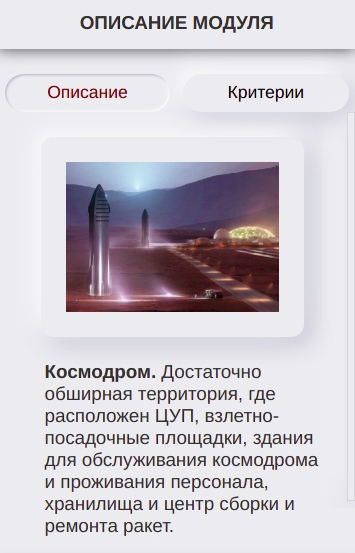
\includegraphics[width=.7\linewidth]{./img/module_description-1}
		\caption{Описание модуля}\label{fig:module_description-1}
	\end{minipage}
	\begin{minipage}{.48\textwidth}
		\centering
		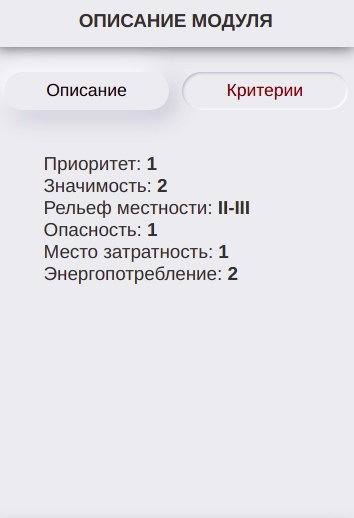
\includegraphics[width=.7\linewidth]{./img/module_description-2}
		\caption{Критерии размещения модуля}\label{fig:module_description-2}
	\end{minipage}
\end{figure}

Как видно из рис.~\ref{fig:module_description-1} в первой вкладке можно найти название модуля, его изображение и текстовое описание. Тогда как во второй (см.~рис.~\ref{fig:module_description-1}) -- уровни критериев размещения.



\subsubsection{Блок <<Дороги>>}

Это последний блок интерфейса программы, где есть только инструменты для размещения, редактирования и удаления дорог на карте.

\begin{figure}[h!]
	\centering
	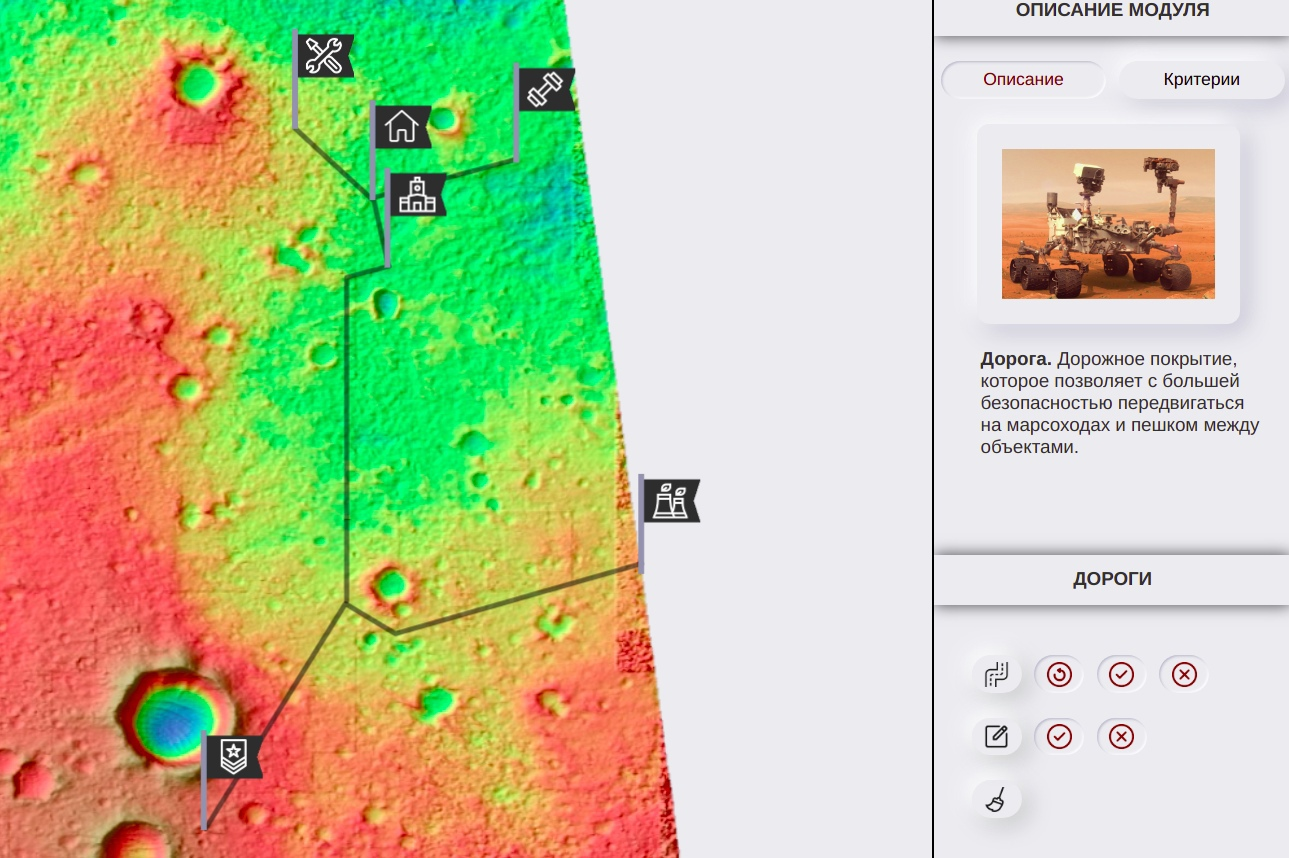
\includegraphics[width=.5\linewidth]{./img/roads}
	\caption{Блок интерфейса <<Дороги>>}\label{fig:roads}
\end{figure}

Начнем с первых инструментов, что вам доступны в первой строке:

\begin{enumerate}
	\item \textbf{Дороги для марсоходов.} Нажатие на эту кнопку позволит вам размещать на карте узлы дорог. То есть при нажатии ЛКМ по точке на карте вы установите ,,узел``, а при повторном нажатии ЛКМ в другом месте второй, они соединятся пунктирной линией, которая символизирует дорогу. Количество узлов неограниченно.
	
	\begin{figure}[h!]
		\centering
		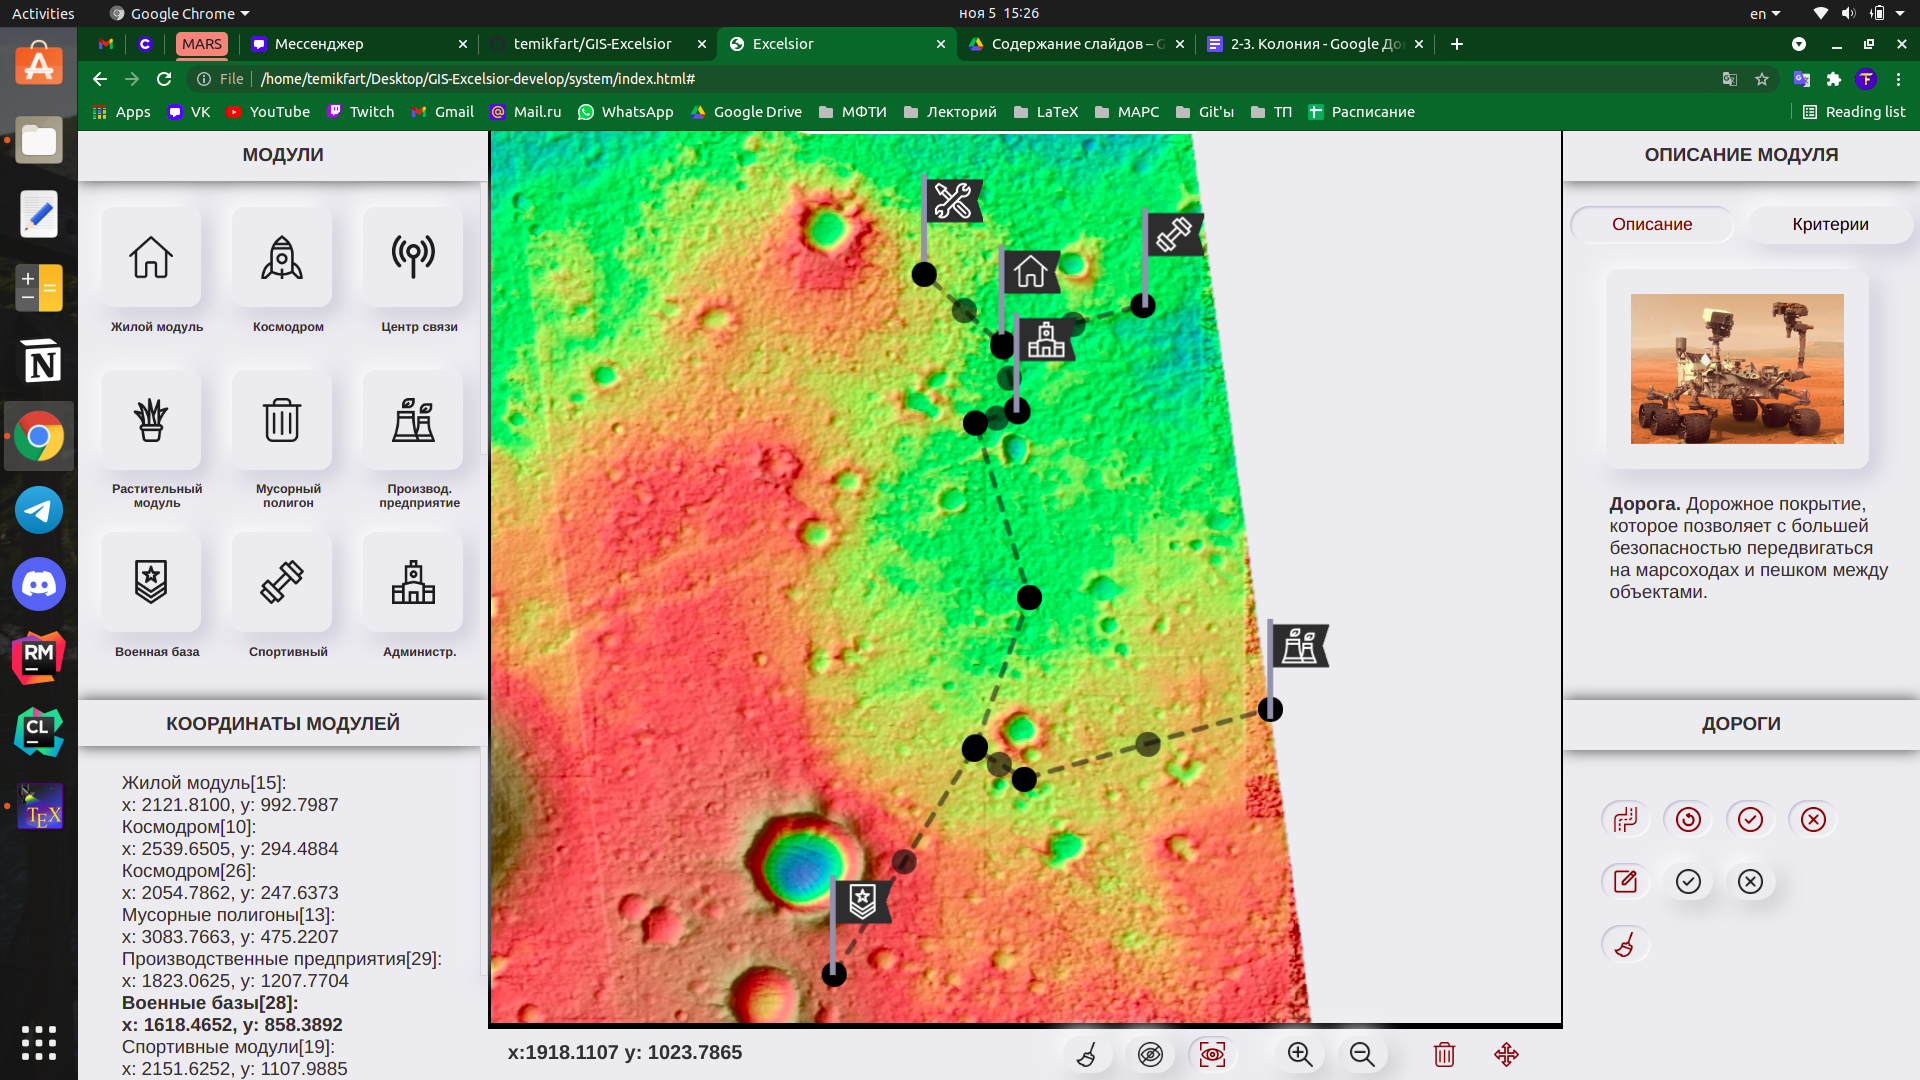
\includegraphics[width=.5\linewidth]{./img/roads_demonstration}
		\caption{Демонстрация размещения дороги на карте}\label{fig:roads_demonstration}
	\end{figure}

	\item \textbf{Назад.} Если вы разместили, например, 5 узлов, то при нажатии на кнопку назад, вы удалите последний размещенный узел.
	\item \textbf{Готово.} Если вы закончили строить дорогу, то нажмите на кнопку <<Готово>>, чтобы завершить размещение. Узлы исчезнут, и останется только ломанная линия, символизирующая дорогу для марсоходов.
	\item \textbf{Отмена.} Если вы начали размещать узлы (но не нажимали кнопку <<Готово>>) и решили удалить их все разом, тогда используйте кнопку <<Отмена>>, чтобы удалить всю размещенную вами дорогу.
\end{enumerate}

Второй строкой расположены инструменты для редактирования существующих дорог:

\begin{enumerate}
	\item \textbf{Редактировать дорогу.} Нажав на эту кнопку, на карте появятся узлы дорог, а также несуществующие узлы на середине каждого ребра, соединяющего два соседних существующих узла.
	
	\textit{Примечание: несуществующие узлы полупрозрачны, в отличие от непрозрачных существующих узлов.}
	
	Наведите на существующий узел, который хотите удалить и нажмите ЛКМ, после этого дорога перестроится, а узла больше не будет на карте.
	
	Если вам хочется встроить еще один узел между двумя имеющимися, тогда кликните ЛКМ на ,,мнимый`` узел ребра, после этого он станет обычным. Вы можете его переместить (\textit{Примечание: можно пропустить предыдущий шаг и сразу же начал перемещать этот узел, тогда перестанет быть мнимым и будет расположен в нужном вам месте.}).
	\item \textbf{Сохранить.} Когда вы закончили редактировать дороги, то вам следует нажать на кнопку <<Сохранить>>. После этого вы автоматически выйдите из режима редактирования дорог и на карте они снова будут отображаться как ломанные линии.
	\item \textbf{Отмена.} Если вы начали редактировать дорогу намеренно или случайно, при нажатии на эту кнопку все изменения будут отменены, вы автоматически выйдите из режима редактирования и дороги будут выглядеть как первоначальные (до входа в режим редактирования) кривые линии.
\end{enumerate}

В третьей строке вы найдете последний доступный вам инструмент:

\begin{enumerate}
	\item \textbf{Очистить.} \underline{Необратимо} удаляются все дороги, которые были на карте.
\end{enumerate}
%
